%für Sprache, A4 Blatt, float, Grafiken, UTF Codierung, PDF, Color, Seitenabstand, Listings
\documentclass[a4papr,12pt]{article}
\usepackage[utf8]{inputenc}
\usepackage[ngerman]{babel}
\usepackage{graphicx}
\usepackage{float}
\usepackage{textcomp}
\usepackage{pdfpages}
\usepackage{tikz}
\usepackage{hyperref}
\usepackage{geometry}
\usepackage{listings}
\usepackage{color}
\usepackage{grffile}
\usepackage{caption}

%Mathematics
\usepackage{amstext}
\usepackage{amssymb}
\usepackage{amsmath}
\usepackage{amsfonts}
\usepackage{mathrsfs}
\usepackage{mathtools}

%include this before fancy or page style gets messed up bc of geometry
%Seitenabstand A4 Blatt
\geometry{a4paper}
\geometry{top=25mm,bottom=25mm,left=23mm,right=20mm}

% macro to select a scaled-down version of Bera Mono (for instance)
\makeatletter
\newcommand\BeraMonottfamily{%
  \def\fvm@Scale{0.85}% scales the font down
  \fontfamily{fvm}\selectfont% selects the Bera Mono font
}
\makeatother

%Hyperref zum anklicken von Überschriften in Texmaker + Farben einstellen
\hypersetup{
	colorlinks,
	citecolor=black,
	filecolor=black,
	linkcolor=blue,
	urlcolor=black
}

\definecolor{mygreen}{rgb}{0,0.6,0}
\definecolor{mygray}{rgb}{0.5,0.5,0.5}
\definecolor{mymauve}{rgb}{0.58,0,0.82}

%Zum Pascal Code einfügen mit lstinputlisting[language=Pascal] {../blabla.pas}
\lstset{ %
  backgroundcolor=\color{white},   % choose the background color; you must add \usepackage{color} or 								  \usepackage{xcolor}
  basicstyle=\BeraMonottfamily,        % the size of the fonts that are used for the code
  breakatwhitespace=false,         % sets if automatic breaks should only happen at whitespace
  breaklines=true,                 % sets automatic line breaking
  captionpos=b,                    % sets the caption-position to bottom
  commentstyle=\color{mygreen},    % comment style
  deletekeywords={...},            % if you want to delete keywords from the given language
  escapeinside={\%*}{*)},          % if you want to add LaTeX within your code
  extendedchars=true,              % lets you use non-ASCII characters; for 8-bits encodings only, 												does not work with UTF-8
  frame=single,	               % adds a frame around the code
  keepspaces=true,                 % keeps spaces in text, useful for keeping indentation of code 									  (possibly needs columns=flexible)
  keywordstyle=\color{blue},       % keyword style
  language=Octave,                 % the language of the code
  otherkeywords={...},           % if you want to add more keywords to the set
  numbers=left,                    % where to put the line-numbers; possible values are (none, left, 								  right)
  numbersep=5pt,                   % how far the line-numbers are from the code
  numberstyle=\tiny\color{black}, % the style that is used for the line-numbers
  rulecolor=\color{black},         % if not set, the frame-color may be changed on line-breaks within 								  not-black text (e.g. comments (green here))
  showspaces=false,                % show spaces everywhere adding particular underscores; it 														overrides 'showstringspaces'
  showstringspaces=false,          % underline spaces within strings only
  showtabs=false,                  % show tabs within strings adding particular underscores
  stepnumber=2,                    % the step between two line-numbers. If it's 1, each line will be 								  numbered
  stringstyle=\color{mymauve},     % string literal style
  title=\getlstname,
  tabsize=2,	                    % sets default tabsize to 2 spaces
  inputencoding=latin1,
  columns=fullflexible
}

\lstset{literate=%
	{Ö}{{\"O}}1
	{Ä}{{\"A}}1
	{Ü}{{\"U}}1
	{ß}{{\ss}}1
	{ü}{{\"u}}1
	{ä}{{\"a}}1
	{ö}{{\"o}}1
	{~}{{\textasciitilde}}1
}

%Filenamen und Pfad trennen
\makeatletter
\DeclareRobustCommand{\getlstname}{%
\begingroup
  % \lstname seems to change hyphens into \textendash
  \def\textendash{-}%
  \filename@parse{\lstname}%
  \texttt{\filename@base.\filename@ext}%
\endgroup
}


%Für Kopfzeile den Style
\usepackage{fancyhdr}
\pagestyle{fancy}
\lhead{AUD 2\textbackslash PRO 2 - Übung 4}
\rhead{Andreas Roither, \today{}}
\newcommand{\Cross}{\mathbin{\tikz [x=1.4ex,y=1.4ex,line width=.2ex] \draw (0,0) -- (1,1) (0,1) -- (1,0);}}%

\begin{document}

%ANGABE     
\thispagestyle{plain}
\includepdf[pages={1},pagecommand={     
\begin{tikzpicture}[remember picture, overlay]\node at (15.8, -0.85) {6 h};\end{tikzpicture}
\begin{tikzpicture}[remember picture, overlay]\node at (7.6, -0.85) {Andreas Roither};\end{tikzpicture}
\begin{Huge}
\begin{tikzpicture}[remember picture, overlay]\node at (-1.3, -1.9) {X};\end{tikzpicture}
\end{Huge}
}]{Angabe/UE4.pdf}
\thispagestyle{plain}
%\includepdf[pages=2-,pagecommand={}]{Angabe/UE4.pdf}

\section*{Übung 4}
\subsection*{Aufgabe 1}
\subsubsection*{Lösungsidee}
Auf Basis eines binären Suchbaums wird eine Pascal-Unit erstellt. Diese Unit enthält folgende Operationen:

\begin{itemize}
\item IsEmpty:  \newline Gibt True oder False zurück, je nachdem ob etwas in dem Baum enthalten ist oder nicht
\item Insert:   \newline Ermöglicht es etwas in den Baum einzufügen
\item Remove:   \newline Entfernt eine Node des Baumes
\item Contains:  \newline Gibt True oder False zurück, je nachdem ob ein bestimmter String im Baum enthalten ist
\end{itemize} 

\lstinputlisting[language=Pascal] {../WC_ADS.pas}
\lstinputlisting[language=Pascal] {../WC_ADS_TEST.pas}
\begin{figure}[H]
	\centering
	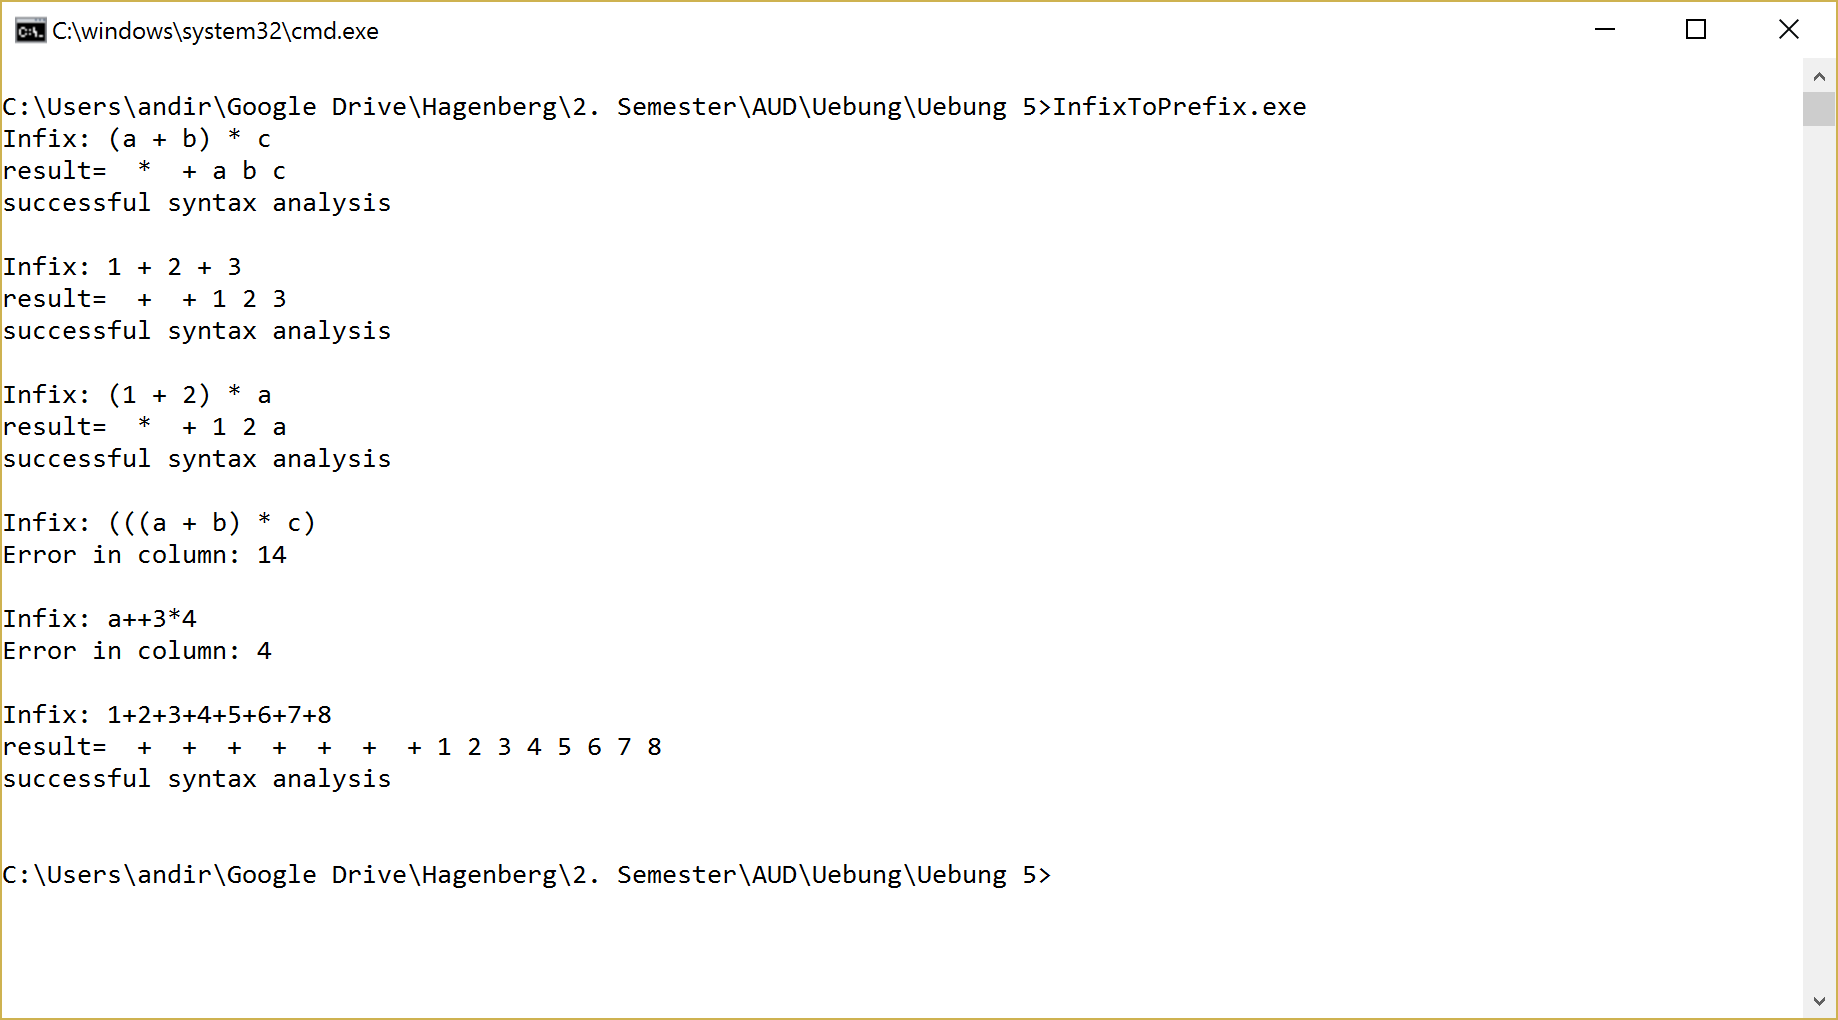
\includegraphics[scale=0.8]{./pictures/1.png}
	\caption{WC ADS Unit Test }
	\label{fig: WC_ADS Unit}
\end{figure}
\raggedright
Die Testfälle zeigen die Verwendung der Funktionen. Bereits vorhandene Wörter werden nicht nochmal eingefügt, deshalb ist trotz neu einfügen des Wortes \grqq{}Hallo\grqq{} und anschließendem löschen und abfragen ob es existiert, \grqq{}Hallo\grqq{} nicht mehr vorhanden. Anders als bei Aufgabe 2 gibt es hier keinen Datentyp auf den zugegriffen werden kann. Anmerkung: Außerhalb der Unit wird es über den Typ Pointer initialisiert aber in der Unit werden TypeCasts zu WordSet ausgeführt.

\newpage
\subsection*{Aufgabe 2}
\subsubsection*{Lösungsidee}
Genau wie Aufgabe 1 nur mit dem Unterschied das ein Typ vorhanden ist auf den zugegriffen werden kann. In dieser Implementation sind die Hintergrund Daten, also \grqq{}Node\grqq{}, nicht sichtbar. Die Operationen funktionieren genau gleich für den Anwender mit der Ausnahme, das ein Objekt mit übergeben werden muss. In der Unit werden TypeCasts bei den Operationen ausgeführt damit der übergebene Pointer verwendet werden kann. Falls also ein anderer Pointer übergeben wird, der auf eine andere Datenstruktur als eine Node zeigt, wird es zu Laufzeitfehlern kommen. Jedoch wird somit sicher gestellt das von außerhalb der Unit nicht auf interne Daten zugegriffen werden kann.
\newline

\lstinputlisting[language=Pascal] {../WC_ADT.pas}
\newpage
\lstinputlisting[language=Pascal] {../WC_ADT_TEST.pas}
\begin{figure}[H]
	\centering
	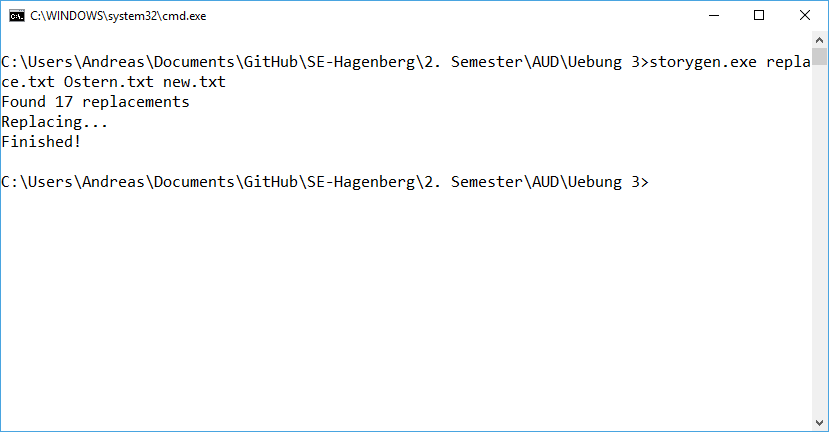
\includegraphics[scale=0.8]{./pictures/2.png}
	\caption{WC ADT Unit Test}
	\label{fig: Matching}
\end{figure}
\raggedright
Zu sehen sind genau die selben Tests wie bei Aufgabe 1. Da sich nur der Zugriff auf die Operationen geändert hat ist hier dasselbe Ergebnis zu sehen. Durch verwenden eines Datentyps können mehrere Objekte existieren die dieselben Funktionen haben. Dadurch können sich zwei Objekte vom Inhalt her unterscheiden. Bei Aufgabe 1 existiert nur ein Objekt innerhalb der Unit. Falls neue Daten eingespielt werden sollen, muss eine Lösch-Operation durchgeführt werden, erst dann können neue Daten eingefügt werden. Bei der Datentyp Variante wird einfach ein neues Objekt erstellt.
\newpage
\subsection*{Aufgabe 3}
\subsubsection*{Lösungsidee}
Ähnlich wie bei Aufgabe 2 werden hier die Daten von Zugriff außerhalb der Unit geschützt. Zusätzlich werden noch weitere Operationen eingefügt:
  \begin{itemize}
\item Union:  \newline Gibt WordSet zurück das alle Nodes (außer Duplikaten) beider WordSets enthält  
\item Intersection:   \newline Gibt WordSet zurück das Wörter enthält die in beiden übergebenen 			WordSets sind
\item Difference:   \newline Gibt WordSet zurück das Wörter enthält die nicht in beiden übergebenen
	WordSets sind
\item Cardinality:  \newline Gibt Anzahl der Elemente im Baum zurück
\end{itemize} 


\lstinputlisting[language=Pascal] {../WS_ADT.pas}
\lstinputlisting[language=Pascal] {../WS_ADT_TEST.pas}
\begin{figure}[H]
	\centering
	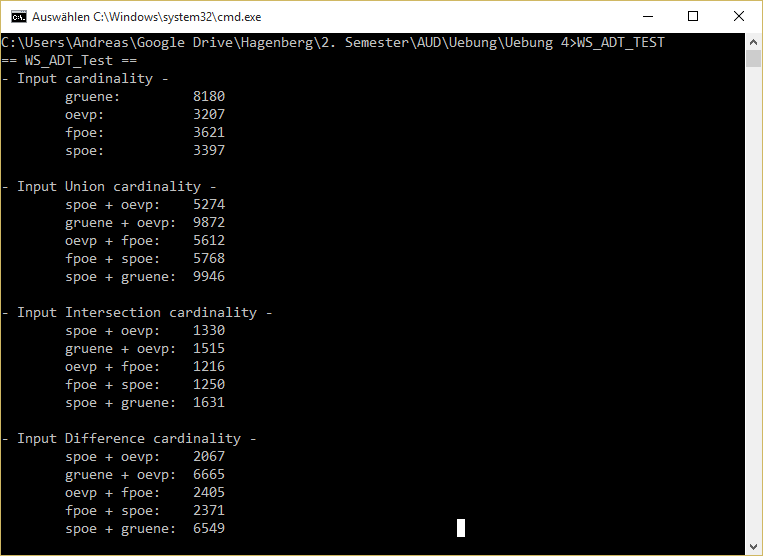
\includegraphics[scale=0.8]{./pictures/3.png}
	\caption{WS ADT Unit Test}
	\label{fig: Matching}
\end{figure}
\raggedright

Bei diesen Testfällen enthält das WordSet von SPÖ und den GRÜNEN die meisten gemeinsamen Wörter, 1631. SPÖ und ÖVP haben \grqq{}nur\grqq{} 1330 gemeinsame Wörter. Hier wird auch ersichtlich das die SPÖ und die GRÜNEN am zweiten Platz stehen bei den unterschiedlichen Wörtern, obwohl sie so viele gemeinsame Wörter haben. Difference gibt das erste übergebene WordSet zurück aus dem alle Wörter entfernt wurden die im ersten und im zweiten übergebenen WordSet entfernt wurden. Anmerkung: Außerhalb der Unit wird es über den Typ Pointer initialisiert aber in der Unit werden TypeCasts zu WordSet ausgeführt.

\end{document}





